\subsection{PIMS Statistics Module}
This module is responsible for displaying statistics from the database. The user has an option to choose the type of graph (either a bar chart or line graph). \par 

\subsubsection{Scope}
The scope is shown in the use case diagram below: \par
\begin{figure}[H]
	\centerline{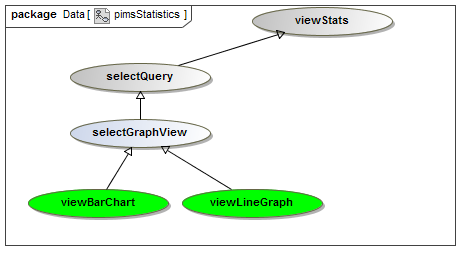
\includegraphics[width=0.7\linewidth]{./Functional_Requirements/Graphics/pimsStats/pimsStatistics}}
	\caption{PIMS statistics module scope}
\end{figure}

\subsubsection{Use cases}
\begin{description}

	\item{\textbf{viewStats -- [priority: critical]}} This use case is a generic version of all statistics to be obtained. Sub-use cases follow the same contract, but return different data.
	\begin{description}
		\item{\textbf{Service Contract}} The generic service contract for all statistics is shown below.
		\begin{figure}[H]
			\centerline{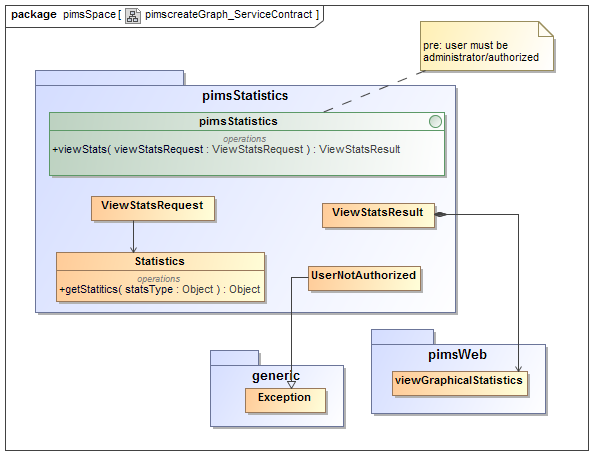
\includegraphics[width=0.7\linewidth]{./Functional_Requirements/Graphics/pimsStats/pimscreateGraph_ServiceContract}}
			\caption{Service contract for viewStats}
		\end{figure}
	\end{description}
		\begin{description}
		\item{\textbf{Process Specification}} The generic process specification for all statistics is shown below.
		\begin{figure}[H]
			\centerline{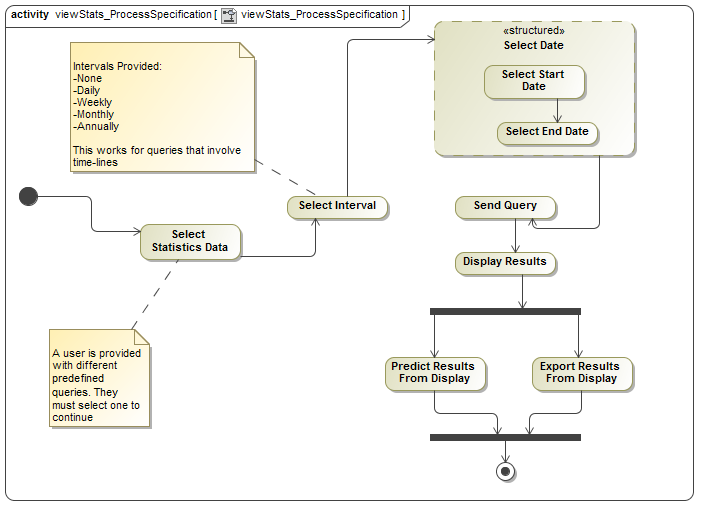
\includegraphics[width=0.7\linewidth]{./Functional_Requirements/Graphics/pimsStats/viewStats_ProcessSpecification}}
			\caption{Process specification for viewStats}
		\end{figure}
	\end{description}
	
		\item{\textbf{createGraph -- [priority: critical]}} This use case creates and displays a graph. This graph can be viewed by the client or downloaded for record keeping.
	
\end{description}
